\chapter{Getting Started with Ravel}

Ravel has three main components:
\begin{itemize}
\item The Ravel, a visual representation of your data;
\item Equations expressed as flowcharts; and
\item The system-dynamics engine Minsky
\end{itemize}

\section{System requirements}

Ravel is a proprietary program for data analysis which currently only runs on Windows. It is built on top of Minsky, which is an open source program available for Windows, Mac OS X,and various Linux distributions. Some components of the interface are specific to Minsky. This "Getting Started" guide focuses on the components used by Ravel. For a getting started guide to Minsky, \htmlref{click here}{Getting-Started-Minsky}.

\section{Getting help}

Press the F1 key, or select ``help'' from the context menu. Help is context-sensitive. If you press F1 while the mouse is hovering over a widget--for example, the addition block--then the help window will appear with instructions on how to add elements together.


\section{Components of the Program}

There are 5 main components to the Ravel interface:

\begin{enumerate}
\item  The menus.

  \begin{tabular}{lllllll}
    File & Edit & Bookmarks & Insert & Options & Simulation & Help \\
  \end{tabular}

\item  The Operations controls

\htmladdimg{OperationsControls.png}

\item The Tabs. 

\htmladdimg{Tabs.png}

These are 

\begin{itemize}
\item Wiring, where a model is defined;
\item Equations, which shows you a bitmapped image of all the equations in your model (to see well-formatted equations, use the "File/Export Canvas As" menu, choose LaTeX as the output format, and load the resulting .TeX file into a LaTeX editor);
\item Summary, which provides a detailed and mathematically formatted table of all the components of your model;
\item "Phillips Diagram", which is a Minsky-specific feature not used by Ravel;
\item "Publication", which is a default blank canvas onto which any component of your model can be placed for documentation purposes; and
\item The "+" tab, which enables you to create and name a new Publication tab. Any number of Publication tabs can be created, which lets you save multiple views of a file for different audiences--the one for auditing, say, would be different to the one for marketing, and so on.

\end{itemize}



\item The design icons. These are "widgets" which are placed on the canvas to perform various operations. These include data import parameters, Ravel objects, plots and sheets for displaying data, mathematical operators for analysing your data, and so on. These are explained in detail in the reference sections of the online help.

\fwhtmladdimg{DesignIcons.png}

\item And finally, the Design Canvas--the large drawing area beneath the buttons and icons.

\fwhtmladdimg{RavelCanvas.png}
\end{enumerate}

Some of the elements of the interface are specific to the simulation engine Minsky--for example, the Record and Replay buttons, the Reverse checkbox, "Run-Stop-Step" buttons and the simulation speed slider. These aspects of the interface are explained in the Minsky section of this manual.

\htmladdimg{RunButtons.png}

Others are used by both Ravel and Minsky--for example, the Recalculate button:

\htmladdimg{Recalc.png}

And the Zoom controls, which enable you to Zoom out and In, go to standard Zoom, and fit the document to the visible screen:

\htmladdimg{ZoomControls.png}

\subsection{Menu}
\label{Menu}

The menu controls the basic functions of saving and loading files, default settings for the program, etc. These will alter as the program is developed; the current menu items (as of April 2024) are: 

  \begin{tabular}{lllllll}
    File & Edit & Bookmarks & Insert & Options & Simulation & Help \\
  \end{tabular}

\subsubsection{File}
\label{File}

\begin{description}
\item[About] Tells you the version of Ravel and/or Minsky that you are using.

\item[New System] Clear the design canvas. If you have made changes and haven't saved them, you will be prompted to save before the canvas is cleared.

\item[Open] Open an existing Ravel or Minsky file (Ravel files have the suffix of "rvl". Minsky files have the suffix of ``mky").

\item[Recent Files]\label{recentfiles} Provides a shortcut to some of your previously opened Ravel (or Minsky) files.

\item[Library] Opens a web-based repository of models for the Minsky simulation system. 

\item[Save] Save the current file.

\item[Save As] Save the current file under a new name.

\item[Insert File as Group] Insert a Ravel/Minsky file directly into the current model as a \htmlref{group}{Group}

\item[Dimensional Analysis] This is a Minsky-specific command to check whether definitions in a simulation model are consistent

\item[Export Canvas as] Export the current canvas in svg, pdf, eps, tex, or m format. The current canvas (which varies depending on which Tab you have open) can be exported in a number of different formats:

\begin{itemize}
\item SVG
This is a "vector graphics" format which can be inserted into word processing (such as Word or OpenOffice) or presentation (Powerpoint etc.) documents.
\item PDF
This saves the currently displayed canvas as an Adobe Acrobat file
\item EMF
This saves the canvas in an enhanced form of the WMF (Windows Metafile) vector graphics standard, for use in documentation programs like Powerpoint and Word.
\item Postscript
This saves the canvas in an encapsulated form of PDF 
\item Portable Network Graphics
This saves the canvas in a bitmap file (PNG) for use in paint and photo programs, etc.
\item LaTeX
This exports the equations in a model in a mathematical formatting language called LaTeX. This file can be imported into mathematics programs like MathType to document the mathematical logic in your model. If you are a LaTeX user yourself, you can load this directly into your preferred LaTeX editor.


If your LaTeX implemention doesn't support breqn, untick the \htmlref{wrap long equations option}{wrap-equations}, which can be found in the preferences panel under the options menu.
  \item Matlab
This exports the model as an "m. file" for importing into the algebraic program Matlab. This enables the analysis and simulation of your model in a MatLab compatible system, such as \htmladdnormallinkfoot{MatLab}{https://en.wikipedia.org/wiki/MATLAB} or \htmladdnormallinkfoot{Octave}{http://www.gnu.org/software/octave/}.


\end{itemize}


\item[Log simulation] This Minsky-specific command outputs the results of simulated variables into a CSV data file for later use in other programs.

\item[Recording] This Minsky-specific command records the states of a model as it is being built for later replay.

\item[Replay recording] This Minsky-specific command replays a recording of model states.

\item[Quit] Exit the program. Ravel will check to see whether you have saved your changes. If you have, the program will close; if not, you will get a reminder to save your changes.

\item[Debugging use] Items under the line are intended for developer use, and will not be documented here.

\item[Redraw] Redraw may be useful if the screen gets messed up because of a display bug (all programs have them!). For example, a bug could cause items on the canvas to be scaled differently. Redraw could overcome this problem without requiring you to exit the program.

\end{description}

\subsubsection{Edit}
\label{Edit}

\begin{itemize}
\item\label{edit:undo} Undo and Redo allow you to step back and forward in your editing history. If you undo a few edits, and then change the model at that point, the undo history is then reset to commence with your new edit. Ravel supports the standard Windows shortcuts of control-Z for undo and control-Y for redo.

\item\label{edit:copy} Cut/copy/paste. Selecting, or lassoing a region of the canvas will select a group of icons, which will be shaded to indicate the selected items. Wires joining two selected items will also be selected. Note that, compatible with X-windows, selecting automatically performs a copy, so the copy operation is strictly redundant, but provided for users familiar with systems where an explicit copy request is required. Cut deletes the selected items. Paste will paste the items in the clipboard as a \htmlref{group}{Group} into the current model. Ravel supports the Windows-standard shortcut keys of control-C for copy, control-X for cut (which deletes the entity at the current location and creates a copy for pasting elsewhere) and control-V for paste.

%begin{latexonly}
\begin{tabular}{ccc}
\resizebox{0.45\textwidth}{!}{\includegraphics{images/selectionExamplePrior.eps}} & 
\raisebox{1.5cm}{$\Rightarrow$} &
\resizebox{0.45\textwidth}{!}{\includegraphics{images/selectionExamplePost.eps}}\\
\end{tabular}
%end{latexonly}
\begin{rawhtml}
<table>
<tr>
<td><img src="selectionExamplePrior.png"></td>
<td><big>&#x21d2;</big></td>
<td><img src="selectionExamplePost.png"></td>
</tr>
</table>
\end{rawhtml}

\item\label{edit:group} Group selection. Create a \htmlref{group}{Group} using the contents of the selection. Groups allow you to organise more complicated systems components into aggregated modules that make the overall system more comprehensible. In Ravel, groups can be used to, for example, collect all the file importing operations into a Group, thus removing these detail of these operations from the top level view. This reduces the complexity of a canvas, which can make it easier for a viewer to focus on the analysis that the program is actually doing.

\end{itemize}

\subsubsection{Bookmarks}
\label{Bookmarks}
Bookmarks store the location and scaling of a model for future reference. This is an alternative to grouping as a means to organize a model. To create a bookmark, move the canvas and zoom it to the level at which all the items you wish to bookmark are visible. Then click on the Bookmark menu and choose "Bookmark this position". Give the Bookmark a name and it will be added to this menu. To move to that location in the model, click on this Bookmark name. Bookmarks can be deleted using the "Delete bookmark" sub-menu.

\subsubsection{Insert}
\label{Insert}

This menu contains all the \htmlref{mathematical operator blocks}{Operations} used in Ravel, and enables you to place those operators on the Canvas. You can get the same effect by clicking on the Design Icons. A Ravel can be inserted from this menu, as can Minsky-specific tools like \htmlref{Godley table items}{godley} and \htmlref{Plots}{PlotWidget}.


\subsubsection{Options}
\label{Options}

The options menu allows you to customise aspects of Ravel and Minsky. At the moment most options pertain to Minsky rather than Ravel, but this will change as Ravel increases in complexity. In this section of the manual we ignore options pertaining only to Minsky; these are covered in \htmlref{Getting-Started-Minsky}{Getting-Started-Minsky}

\begin{description}
\item[Preferences]\mbox{}

\begin{itemize}
\item Number of recent files to display --- this determines how many previously edited files are displayed on the \htmlref{recentfiles}{recentfiles} menu.
\item\label{wrap-equations} Wrap long equations in LaTeX export. If ticked, Ravel \& Minsky will use the LaTeX "breqn" package to produce nicer looking automatically line-wrapped formulae. Because not all LaTeX implementations are guaranteed to support breqn, untick this option if you encounter problems.
\item\label{font} select a font for variable names, parameter names, etc.
\end{itemize}

\item[Background colour] --- select a colour from which a colour scheme is computed.

\end{description}

\subsubsection{Simulation}
These commands are specific to Minsky and control how a model is simulated. They are covered in the Minsky component of this manual.
\subsubsection{Help}
\label{Help}

Provides an in-program link to this manual. Note that pressing F1 will also launch help windows in a context-sensitive way. That is, it will open the relevant help section for whatever object the mouse is currently hovering over. Similarly, each item on the canvas has a help menu item in the context menu relevant for that item.

\subsection{Record/Replay Buttons}
\label{RecReplayButtons}

\htmladdimg{recReplayButtons.png}

These buttons control the recording / replay mode of Minsky. You can record your interactions with Minsky, and replay those interactions for demonstration/presentation purposes. These commands are specific to Minsky and are covered in the Minsky component of this manual.

\subsection{Recalculate button}
\label {Recalculate}

\htmladdimg{recalculate.png}

The recalculate button computes the values of all variables in a model. Ravel will periodically recalculate, but this is a useful option if you wish to immediately see the results of a calculation.

\subsection{Run Buttons}
\label{RunButtons}

\htmladdimg{NewItem15.png}

These commands are specific to Minsky and are covered in the Minsky component of this manual.


\subsection{Speed slider}
\label{Speedslider}

\begin{center}
\htmladdimg{NewItem16.png}
\end{center}

The speed slider controls the rate at which a model is simulated. These commands are specific to Minsky and are covered in the Minsky component of this manual.

\subsection{Zoom buttons}
\label{ZoomButtons}

\begin{center}
\htmladdimg{NewItem17.png}
\end{center}

The Zoom buttons zoom in and out on the wiring canvas. The same functionality is accessed via the mouse scroll wheel. The reset zoom button \buttonIcon{zoomOrig.eps} resets the zoom level to 1, and also recentres the canvas. It can also be used to recentre the equation view.

The Zoom to Fit button zooms the model so that it just fits in the current canvas window.

\subsection{Simulation time}
\label{SimTime}

In the right hand top corner is a textual display of the current simulation time $t$, and the current (adaptive) difference between iterations $\Delta t$. This information is specific to a Minsky simulation model.

\subsection{Wiring and Equations Tabs}
\label{WiringEquationsTab}\label{tabs:wiring}

\htmladdimg{WiringEquationsTab.png}

This allows you to switch between the visual block diagram wiring view and other views of your document.

\begin{itemize}
\item[Wiring]
This is Ravel's design canvas, where you import data, analyse it using Ravel's mathematical operators and functions, and produce visualisations using Plots and Sheets.
\item[Equations]
As you analyse a model using the flowchart operators in Ravel, the program converts the flowchart logic into standard mathematical formulas. This Tab gives you an instant view of the mathematical logic in your model.
\item[Summary]
This tab provides a structured view of all the equations in a model, with details about the number of dimensions and values in a formula.

For example, this model imports data from the Bank of International Assessments, separates the data into a number of variables, and uses data on debt in domestic currency and debt as a percentage of GDP to derive GDP in domestic currency data.

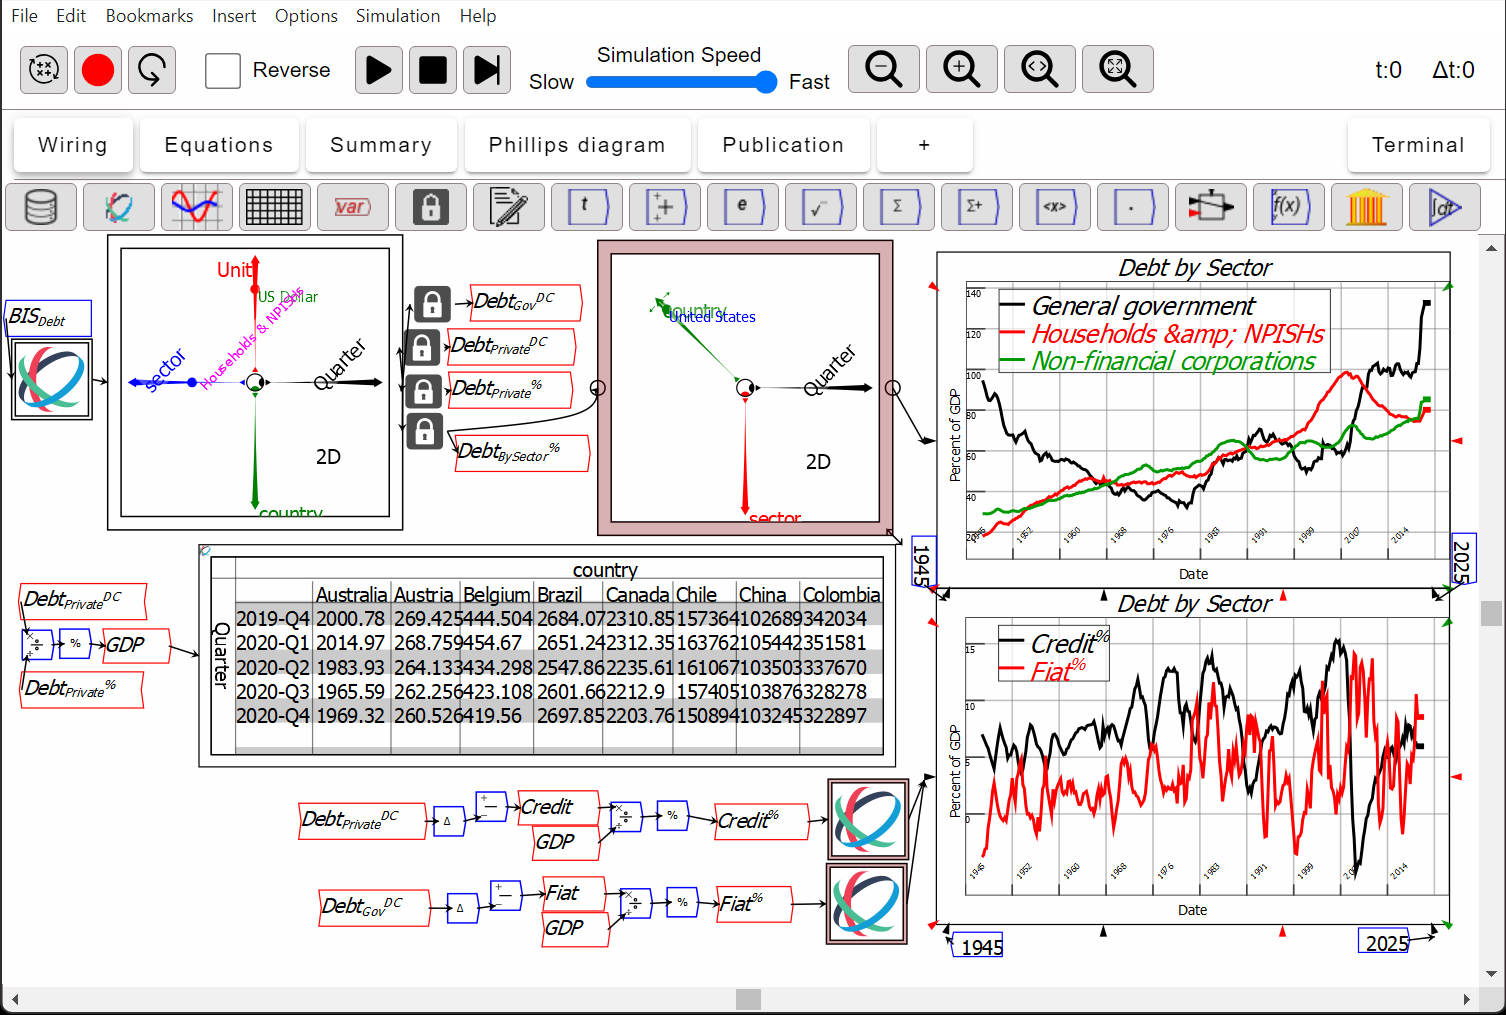
\includegraphics{images/DebtCalcGDPexample.png}

This is the Summary Tab for that model, showing the variable names, their mathematical definitions, their dimensions, and any initial values assigned to them.

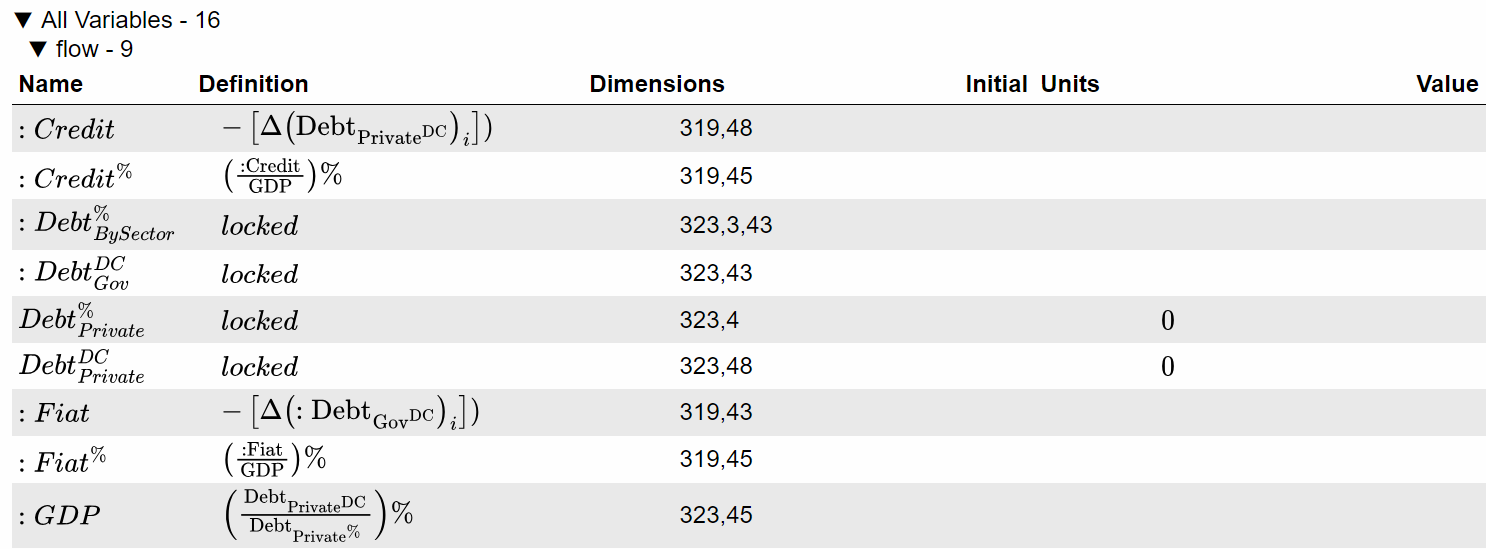
\includegraphics{images/DebtCalcGDPexampleSummaryTab.png}

\item[Phillips Diagram]
This is a Minsky-specific feature which is covered in the Minsky section of this manual.
\item[Publication]
Publication Tabs allow you to place specific items from the Wiring diagram onto a documentation canvas. The default Tab is called "Publication", and additional user-named Tabs can be added using the "+" Tab.

To place an item on a Publication Tab, right-click on it on the Wiring Tab, and then click on "Add item to a publication tab". Click on the desired named tab from the resulting menu. The item will then be placed in the top-left-hand corner of the selected Tab. You can then place it wherever you want on the Publication Tab.

\item[+]
This creates a new tab. Provide a name in the form and press Enter or click OK and the new Tab will be created.
\end{itemize}


\subsection{Design Icons}

\fwhtmladdimg{NewItem18.png}

These are the ``nuts and bolts'' of data analysis using Ravel, and model-building using Minsky. There is a substantial number of icons, and this number will grow over time as more data analysis features are added.

The essential icons for Ravel are the first two: Import Data \buttonIcon{importData.eps} and insert a Ravel \buttonIcon{RavelIcon.png}. 

\begin{description}
\item[Import data] \buttonIcon{importData.eps} Opens an import CSV file dialog, which allows a CSV file to be loaded into a parameter in Ravel (the default name of the parameter is the name of the file being imported). See \htmlref{Importing CSV files}{Operation:csvImport} for full details. After a data file is imported, the next step is to attach it to a Ravel.

\item[Ravel] \buttonIcon{RavelIcon.png}. This places a Ravel on the wiring canvas. The first time this is done in a document, the Ravel is displayed full-size in Edit mode. Subsequent Ravels are displayed in icon mode. For full details on using a Ravel see \htmlref{Ravel}{Ravel}.
  
\item[Plot widget] \buttonIcon{plot.eps} Add \htmlref{plots}{PlotWidget} to the canvas.

\item[Sheet widget] \buttonIcon{sheet.eps} Add a \htmlref{sheet}{Sheet} to the canvas.

\item[Variable]  \buttonIcon{var.eps}. \label{Variable}

This is a pop-up menu, which gives access to the form that creates variables, constants and parameters, and access to the Browser, which is a window that lists all the variables and parameters in a model, and enables them to be placed on the wiring canvas.

Variables are entities whose value changes as a function of time and its relationship with other entities in your model. Click on it and a variable definition window will appear:

\begin{center}
\scalebox{0.5}{\htmladdimg{NewItem32.png}}
\end{center}

The only essential step here is providing a name for the Variable.

Ravel supports the LaTeX language for naming variables (and parameters), which enables you to:

\begin{itemize}
\item Use subscripts and superscripts. The character following an underscore character \_\ is subscripted, while the character following a caret symbol \^\ is superscripted. If the \_\ or \^\ is followed by text in parentheses (curly brackets) \{\}, then all the text within the parentheses is superscripted or subscripted; and
\item Use Greek characters. The English name for a Greek letter (alpha, beta, gamma), preceded by a backslash character $\backslash$ generates the equivalent Greek letter as part of a variable's name  ($\alpha, \beta, \gamma$);

\end{itemize}

This enables more readable variables to be defined, such as, for example $\Delta{Sales}_{Product}^{State}$.

You can also enter a value for it (and a rotation in degrees), but these can be omitted. In a dynamic model, the value will be generated by the model itself, provided its input is wired.


When you click on OK (or press Enter), the newly named variable will appear in the top left hand corner of the Canvas. Move the mouse cursor to where you want to place the variable on the Canvas, click, and it will be placed in that location.


Constants are entities whose value is unaffected by the simulation or other entities in the model. Click on it and a constant definition window will appear:

\begin{center}
\scalebox{0.5}{\htmladdimg{NewItem34.png}}
\end{center}

The only essential element here is its value. You can also specify its rotation on the Canvas in degrees. You can vary the value of a constant or parameter using the arrow keys or the slider button on top of a constant or parameter.

A constant is just a type of variable, which also include parameters (named constants), flow variables, stock variables and integration variables. In fact there is no real conceptual difference between creating a constant or creating a variable, as you can switch the type using the type field.

Like the variable and constant button, the parameter button creates a variable defaulting to the parameter type. Parameters differ from flow variables in not having an input port, and differ from constants in having a name and being controllable by a slider during simulation.

\item[Lock] Lock widgets \buttonIcon{LockIcon.png} are used with \htmlref{Ravels}{Ravel}. A lock keeps a record of the current state of a Ravel: the items selected on its axes, the effect of calipers in selecting data ranges, and so on. You can then manipulate the Ravel without changing the output from the Lock, which can be assigned to a variable for further use. You can also impose the state of a Lock on its associated Ravel.

\item[Notes] Add \htmlref{textual annotations}{Notes}

\item[Time] \buttonIcon{time.eps} embeds a reference to the simulation time on the Canvas. This is a Minsky-specific feature.

\item[Binary operations] \buttonIcon{BinaryButton.png}. These execute the stated binary mathematical operations: operations that require two (or more) inputs. Where appropriate, each input port to a binary operator can take multiple wires---so that to add five numbers together, for example, you can wire 1 input to one port on the Add block, and the other four to the other port. The same applies to the subtract, multiply, and divide blocks: multiple inputs to the input ports on the subtract operator are added together, and then the sum of inputs attached to the "-" port is subtracted from the sum of the inputs attached to the "+" port. For the divide block, the product of the inputs to the "*" port is divided by the product of the inputs to the "/" port.

\htmladdimg{BinaryOperators.png}


Min \& Max Functions. These take the minimum and maximum values, respectively. These also allow multiple wires per input. The sum of the inputs to one port is compared to the sum of the inputs on the other.

Pow and log. These are binary operations (taking just two arguments). In the case of the power operation, the exponent is the top port, and the argument to be raised to that exponent is the bottom port. This is indicated by the $x$ and $y$ labels on the ports. In the case of logarithm, the bottom port (labelled $b$) is the base of the logarithm.

Logical Operators $<$ $\le$, =, $\wedge$ $\vee$ $\neg$ (and, or, not)] These return 0 for false and 1 for true.

\item[Unary functions]\buttonIcon{sqrt.eps} These are a fairly standard complement of mathematical functions which take only one input--though this input can have multiple dimensions.

\item[Reduction operations]\buttonIcon{sum.eps} This menu contains operations that reduce a vector to a scalar, or reduce the rank of a tensor. Typically sum, product, any, all etc.

\item[Scans]\buttonIcon{runningSum.eps} These are running sums and the difference operator

\item[Miscellaneous tensor operations]\buttonIcon{outerProduct.eps}
  Any other tensor function not covered elsewhere.

\item[Switch] \buttonIcon{switchIcon.eps} Add \htmlref{a piecewise-defined function block}{SwitchIcon} 
to the canvas. Also known as a hybrid function.

\item[User defined function]\buttonIcon{userFunction.eps} You can
  define \htmlref{your own function}{Operation:userFunction} using an algebraic expression, such as \verb+exp(-x^2+y)+.

\item[Godley Table] \buttonIcon{NewItem29.eps}. \label{GodleyTable} This is the fundamental element of Minsky that is not found (yet) in any other system dynamics program. It is covered in the Minsky chapter of this manual.


\item[Integration] \buttonIcon{int.eps}.\label{Integrate}
  This inserts a variable whose value depends on the integral of other variables in the system. It is discussed further in the Minsky section of the manual.
  
\item[Derivative Operator] \buttonIcon{differentiate.eps} This operator symbolically differentiates its input. It is a component of Minsky which is explained in the Minsky section of this manual.

\end{description}

\subsection{Design Canvas}
\label{DesignCanvas}\label{tabs:Wiring}

The Design Canvas is where you develop your model. A model consists of a number of blocks---imported data in parameters, Ravels, user-defined parameters, variables, constants, mathematical operators and the display elements (plots and sheets)---connected by wires. 

The canvas is {\em zoomable}, either via the zoom buttons on the toolbar, or via the mouse scroll wheel. It is also {\em pannable}, either via the
scroll bars on the right and bottom, or by holding the shift key and left mouse button together. The canvas is effectively unlimited, however the scroll bars treat the canvas as a $10000\time10000$ pixels in size.

\fwhtmladdimg{NewItem19.png}

\subsection{Equations tab}\label{tabs:Equations}

This displays the mathematical representation of the model

\subsection{Summary Tab}\label{tabs:Summary}

This tab provides a summary table of all variables in the system, in a
heirarchical fashion that can be navigated by expanding or hiding
sections by toggling the caret. Each variable shows its name, it
definition, dimensions (for tensor-valued variables), initial
expression, units and current value.

Most of these fields are editable, and usually do the obvious
thing. Changing a variable's name will do a {\em replace all
  instances} operation to update all variables of the same
name. Changing a variable's definition will replace the wiring graph
leading into the variable by a \htmlref{user defined function}{UserFunction} containing your
edited string. At some future point, functionality will be added to
convert a user defined function into a wiring graph.

\subsection{Phillips diagram tab}\label{tabs:Phillips}

This tab implement's Minsky's take on a \htmladdnormallink{Phillips
  diagram showing the stocks and flows in a monetary
  economy}{https://en.wikipedia.org/wiki/Phillips_Machine}. The
Phillips tab shows all the information contained in the Godley tables
of the model - if there aren't any, this tab will be blank.

Initially, all the stocks will be arranged around a circle, with the
flows shown as connecting arrows showing the current direction of the
flow. You can move and rotate the stocks, and bend the flows to make a
pleasing layout. The stocks will be coloured as though filled with a
fluid like Bill Phillip's original analogue computer, and dynamically
updated as the simulation proceeds.

\subsection{Publication tab}\label{tabs:Publication}

Publication tabs allow the creation of dashboards to emphasise certain
aspects of a simulation. For example, you may wish to focus on a
particular plot or Godley table when running the simulation.

Multiple publication tabs can be created by clicking the '+' tab.

Any item from the wiring tab can be added to a publication tab, and
then moved, resized or rotated independently of the item on the wiring
tab. For items that dynamically update, the publication tab will be
updated dynamically during the simulation.

Textual annotation can be added to the publication tab, independently
of any annotations on the wiring tab.

Wires cannot be added to the publication tab, however you can insert
arrows (eg $\rightarrow$) by typing the LaTeX text \verb+\rightarrow+,
and then rotate and scale the arrow to connect parts of the dashboard together.

\subsection{Wires}
\label{Wires}

The wires in a model connect blocks together to define equations. For example, to write an equation for 100/33, you would place a \buttonIcon{const.eps} on the canvas, and give it the value of 100:

\begin{center}
\scalebox{0.5}{\htmladdimg{NewItem122.png}}
\end{center}

Then do the same for 33, and place a divide block on the canvas:

\begin{center}
\includegraphics{images/NewItem123.eps}
\end{center}

Then click on the right hand edge of \buttonIcon{const100.eps} and drag to extend the wire to the numerator ($\times$) port of the divide operation.

\begin{center}
\includegraphics{images/wireExample1.eps}
\end{center}

Finally, add the other wire.
\begin{center}
\includegraphics{images/wireExample2.eps}
\end{center}

\section{Working with Ravel}

\subsection{Components in Ravel}

There are several types of components in Ravel
\begin{enumerate}
\item Data storage parameters, which load in data from an external CSV file;
\item Ravels, which take data from a data storage parameter and create a multi-dimensional graphical rendition of the data, with one axis per dimension;
\item Mathematical operators such as plus (+), minus (-), etc. These are all aware of the dimensions of your data, so they act on arrays of data, rather than single cells as with spreadsheet formulas;
\item Constants (or parameters, which are named constants) which are given a value by the user;
\item Variables whose values are calculated by the program during a simulation and depend on the values of constants and other variables; and
\item Groups, which allow components to be grouped into modules that can be used to construct more complex models.
\end{enumerate}


\subsection{Inserting a model component}


There are five ways to insert a component onto the Canvas:
\begin{enumerate}
\item Click on the desired Icon on the Icon Palette, drag the block onto the Canvas and click the mouse where you want to insert it 

\begin{center}
\fwhtmladdimg{NewItem18.png}
\end{center}

\item Choose Insert from the menu and select the desired block there

  \begin{center}
    %begin{latexonly}
    \resizebox{!}{0.6\textheight}{
      %end{latexonly}
      \htmladdimg{NewItem159.png}
     %begin{latexonly}
    }
    %end{latexonly}
  \end{center}
  \newpage
  
\item Right-click on an existing block and choose copy. Then place the copy where you want it on the palette. 

\begin{center}
\htmladdimg{NewItem161.png}
\end{center}

\item Variables can be inserted by typing the variable name on the canvas, and constants can be entered simply by typing the number on the canvas. Similarly, operations can be inserted by typing the operator name (eg \verb+sin+, or \verb+*+). Notes can be inserted by starting the note with a \verb+#+ character.

\item Variables can also be picked from the \htmlref{Variable
    Browser}{VariableBrowser} and placed on the canvas.
\end{enumerate}


\subsection{Creating an equation}

Equations are entered in Ravel graphically. Mathematical operations like addition, multiplication and subtraction are performed by wiring the inputs up to the relevant mathematical block. The output of the block is then the result of the equation. 

For example, a simple equation like
\begin{displaymath}
100/3 = 33.3
\end{displaymath}
is performed in Minsky by defining a constant block with a value of 100, defining another with a value of 3, and wiring them up to a divide-by block. Then attach the output of the divide block to a variable, and run the model by clicking on\smhtmladdimg{NewItem130.png} :

\begin{center}
  \includegraphics{images/NewItem129.eps}
\end{center}

If you click on the equation tab, you will see that it is:

\begin{displaymath}
\mathrm{Answer}=\frac{100}{3}
\end{displaymath}

\subsection{Wiring components together}

A model is constructed by wiring one component to another in a way that defines an equation. Wires are drawn from the output port of one block to the input port of another. Ports are circles on the blocks to which wires can be attached, which can be seen when hovering the pointer over the block. Variables have an input and an output port; constants and parameters only have an output port. A mathematical operator has as many input ports as are needed to define the operation.

To construct an equation, such as Fred - Wilma = Barney:

Click the mouse near the output port of one block and drag the cursor to the input port of another while holding the mouse button down. An arrow extends out from the output port. Release the mouse button near the required input port of the operator. A connection will be made.

\begin{center}
\includegraphics{images/NewItem181.eps} 
\end{center}

The equation is completed by wiring up the other components in the same way.

\begin{center}
\includegraphics{images/NewItem182.eps} 
\end{center}
